%!TeX root = main.tex
\documentclass[main.tex]{subfiles}

\begin{document}

\chapter{Database approach}\label{database}
\clearpage

\section{Screening studies}

Research on the adsorption properties of zeolites in particular, and nanoporous materials in general, aims at understanding the nature and respective importance of the different interactions that drive the adsorption phenomenon. This understanding can afterwards be turned into principles, which are then applied to predict the adsorption capacities of similar materials on similar gases, where these principles remain valid.

The natural starting point for this research is a study of a particular material with a particular gas, which leads to particular observations that may then be generalized. Many such studies have been performed and published on zeolites, each involving a considerable amount of work, which provide very precise results on a given topology, with up to a few different \SiAl ratios. Yet, the conclusions can seldom be carried over to provide predictions on other topologies.

The converse strategy consists in doing screening studies, in which a vast array of structures is tackled at the same time. Given the cost of doing so experimentally, these studies are mostly computational, thus providing less precise results than actual experiments, but on a broader scale.

Most zeolite screening studies focus on all-silica zeolites, an approach that sidesteps the issue of placing aluminium and cations. However, most zeolite adsorption applications require cationic zeolites, since cations critically increase the adsorption capacity of the materials.

Even among the few studies which tackle cationic zeolites across topologies and \SiAl ratios, not all properly place cations in the framework, although it is known that this can lead to incorrect subsequent adsorption measurements \autocite{Fang2016}. For example, \textcite{Mousavi2023} target 57 different topologies with 5 different possible cations, but fail to mention where these are placed before the start of the Grand Canonical Monte Carlo (GCMC) simulations, likely resulting in them being trapped in a non-optimal placement. \Textcite{SmitNature2012} also screens cationic zeolites, but place cations at the so-called ``minimum energy positions'' instead of using a robust method like parallel tempering; they also use a force field made for FAU zeolites only, which is inadequate to screen other zeolites.
%I am only aware of the works of \cite{Fang2016}, which tackles many zeolite with various \SiAl ratios for screening purposes, that properly places cations through parallel tempering.

In this chapter, I explain how I constitute a database of cationic zeolite structures and how it can be used for isotherm prediction through statistical methods. This work is ongoing at the time of writing.

\section{Adsorption isotherm}

\subsection{Definition and classification}

\label{isotherms}

The behaviour of a material with respect to the adsorption of a gas is typically assessed by measuring the evolution of its adsorption capacity with external fluid pressure, at a fixed temperature. The resulting curve is called an isotherm, and it is usually classified according to its general shape into one of several possible categories, represented on \cref{fig:IUPACisotherms}.

The shape of the isotherm depends on the surface of the material, the strength of its interaction with the adsorbate and of the adsorbate-adsorbate interactions. For example, type I isotherms are often observed on materials with very small external surface and monodisperse pores of small size, where adsorption quickly reaches saturation. On the other hand, type III isotherms occur when the adsorbent-adsorbate interaction is weak and adsorption is not limited by the pore size (either because adsorption occurs on the external surface or because the pores are very large). Some of these types exhibit hysteresis loops: for example, type IV(a) isotherms, typical of mesoporous adsorbents, have the adsorption branch lower than the desorption branch (when the gas is withdrawn), which comes from the capillary condensation of the adsorbate at high pressure. Real isotherms are often combinations or slight variations of these idealized types \autocite{BrandaniIsotherms2016}.

At very low pressure, all isotherms are expected to be linear: this is Henry's law, and Henry's adsorption constant $K$ is proportional to the slope of the isotherm. In that limit, all adsorbates behave like ideal gases since, by definition, there is no adsorbate-adsorbate interaction at low enough pressure.

\begin{figure}[t]
	\centering
	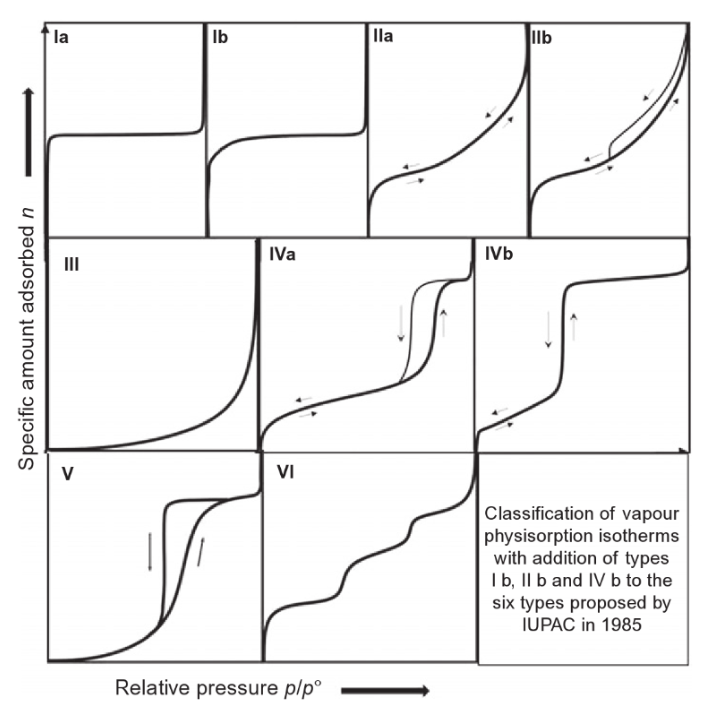
\includegraphics[width=0.6\columnwidth]{figures/database/IsothermTypes.png}
	\caption{Classification of gas isotherm by IUPAC, taken from \cite{Rouquerol2013}, itself adapted from \cite{IUPAC1985}. $p^0$ designates the saturation pressure of the adsorbate.}\label{fig:IUPACisotherms}
\end{figure}

The other end of the pressure spectrum is more complex. When adsorption occurs on the external surface of the adsorbent, for instance with clays, and if adsorbent-adsorbent interactions are strong enough to allow multi-layer adsorption, then the number of adsorbed species never stops growing with increasing pressures. However, with zeolites and more generally any adsorbent where adsorption occurs in finite pores, the adsorption capacity plateaus at high pressure when all the pores are filled with the adsorbate. It should be mentioned though that the adsorption capacity can still increase beyond that limit, because of the compressibility of the adsorbate in liquid or supercritical state. These regimes of extremely high pressure (above $\qty{100}{MPa}$) are of lesser industrial relevance because reaching these conditions is costly and hazardous. They are, however, visible in simulations.

\subsection{Experimental observation and numerical prediction}

\label{experimentalisotherm}

Experimentally, adsorption isotherms are measured by progressively increasing the input pressure of the adsorbate in the material at the fixed temperature, and measuring the amount adsorbed. The desorption isotherm follows up by progressively decreasing the input pressure, and similarly measuring the amount of adsorbate.

The measurement itself usually consists in either of the three following methods \autocite{BrandaniIsotherms2016}:
\begin{itemize}
	\item volumetry: a fixed amount of gas at the target pressure is put in contact with the adsorbent, and what is measured is the difference of pressure before and after adsorption.
	\item breakthrough: the gas starts flowing through the adsorbent at a given time, and the outlet concentration and volumetric flowrates are measured.
	\item gravimetry: the difference in mass of the sample containing the adsorbent before and after adsorption is measured by balancing its weight against buoyancy.
\end{itemize}
By reproducing the experiment with a reference gas (usually \ce{N_2} or \ce{Ar}), these techniques give access to the net adsorption, which is the absolute amount of adsorbed species minus that which would be in a fluid occupying the same space as the adsorbent at the same pressure and temperature. Knowledge of the volume of adsorbent allows retrieving the absolute adsorption capacity, which is the thermodynamic variable directly accessible in simulations.

Some more anecdotic isotherm measurement techniques including impedance spectroscopy as well as NMR allow obtaining directly the absolute adsorption \autocite{BrandaniIsotherms2016}, but these methods are much too costly to be used routinely.

The adsorption capacity can be predicted numerically through GCMC simulations, as explained in \cref{GCMC}. Beyond the limits due to the precision of the energy computation, either from a force field or from DFT, and convergence of the simulations, those are also dependent on a model of the adsorbent, which cannot take into account the complexity of real materials. In the case of zeolites, the location of the aluminium and of the cations has already been discussed through \cref{cationzeolites}, but more generally, all kinds of defects and small crystal size effects can lead to experimental isotherms differing from the simulated counterparts. This limits the accuracy of individual numerical simulation compared to precise experiments. They remain useful however to extract tendencies and direct the search for new adsorbents, which may be experimentally tested eventually.

\section{Database constitution}

Finding general tendencies in the adsorption behaviour across zeolites requires doing the analysis of many different structures. To do so, the first step consists in establishing a database of models for the materials themselves. The general workflow for creating these structures, starting from the idealized zeolite structure defined by its topology, down to the cation placement, has already been described in \cref{cationzeolites}. To summarize, the two steps are:
\begin{enumerate}
	\item Aluminium placement. Start by finding the minimum \SiAl ratio by replacing as many silicon with aluminium atoms as possible, with random exchanges and restarts. Check multiple supercell sizes. Then, starting from these filled structures, replace some aluminium by silicon atoms at random and do more exchange steps to generate 6 aluminium placements for each target \SiAl ratio.
	\item Cation placement: using either parallel tempering or ``shooting star'' simulations, combined with annealed site hopping once the sites are localized. The only cation used in the current study is sodium.
\end{enumerate}

For the entire database, I used the same force field which is that developed by \textcite{BoulfelfelSholl2021} for the adsorption of small gases on cationic zeolites with mobile cations. As with any force field, it has limited accuracy, but the goal is to develop and test a methodology with a fixed known force field to ensure the consistency of the database.

\subsection{Aluminium placement}

The current database contains 6 aluminium placements for all 239 known and not interrupted zeolite topologies, with \SiAl ratios of \num1, \num{1.23}, \num{1.4}, \num{1.7}, \num{2}, \num{3}, \num{5} and \num{10}. The actual \SiAl ratios of each structures are those closest to the previous references, which may sometimes differ. When the minimum \SiAl ratio (presented in \cref{table:zeosial}) is not among the previous references, it is added separately, and the lower \SiAl ratios cannot be generated. For example, the list of actual \SiAl ratios for topology YUG is $1.56$, $\frac{121}{71}\approx1.704$, $2$, $3$, $5$ and $\frac{349}{35}\approx9.971$.

The algorithm sometimes fails at finding 6 distinct aluminium placements, because of high symmetry constraints: in that case, the maximum number of distinct placements is kept.% To check whether a new placement is distinct from previous ones, the following algorithm is used. First, for each topology, the list of T-sites is mapped to the list of integers between $1$ and $N$, the number of T-sites of the topology. Each placement is represented by a sequence of $N$ bits, where a bit of 1 at position $i$ indicates an aluminium in T-site $i$ and 0 stands for silicon. Then, all $M$ symmetries of the topology are applied to the placement: this results in $M$ $N$-bit sequences. The (lexicographically) smallest among those serves as a unique signature that identifies the aluminium placement. When a new placement is found, is signature is computed as previously and compared to those already encountered: if it is different from all of them, the new placement is stored.
In the case where $\SiAl = 1$ for example, there can be up to only 2 distinct aluminium placements that obeys L\"owenstein's rule: taking an arbitrary T-atom as a reference, one placement corresponds to that reference set to Al, and the other to that reference set to Si. For many topologies, these two placements are actually symmetry-equivalent, so they share the same signature and only one of them is actually stored. This is not necessarily the case however: for example, topology JSW has two distinct aluminium placements for $\SiAl = 1$.

Overall, \num{8983} different structures with aluminium placed were generated. Each of these then need to have extra-framework cations in order to represent an electrically neutral material.

\subsection{Cation placement}

For all 239 known and non-interrupted topologies, and for each of the up to 6 different aluminium placements corresponding to the minimum \SiAl, a ``shooting star'' simulation was launched with the hot run at \qty{2000}K for \num{20000} cycles (and \num{2000} initialization cycles), spawning one cold simulation every \num{100} cycles. Each of the resulting \num{200} cold simulations ran at \qty{300}K for \num{10000} cycles. This served as an experiment to assess the convergence of the simulations: out of the 239 topologies, 57 converged in less than \num{5000} cycles (averaged across aluminium placements). For these topologies only, ``shooting star'' simulations were run for all previously created aluminium placements across the different \SiAl ratios, using the same parameters (except for the number of cold cycles raised to \num{15000}). For each ``shooting star'' simulation, the \num{200} cold simulations are divided into six groups, and for each of these groups, the structure with the lowest corresponding energy is kept. Hence, this methodology yields 6 cation placement per structure.

This methodology is a reduced version of the full cation placement strategy illustrated on the FAU topology in \cref{casestudyFAU}. Such a strategy starts by identifying cationic sites using the previous simulation results, then follows up by running site hopping simulations augmented by simulated annealing (or another meta-algorithm) for each desired \SiAl ratio and aluminium placement. This ensures the optimal repartition of the cations in the different sites, although the site locations themselves may not be perfectly adequate for each precise structure, since they are identified based on a cation density map averaged over different structures. The 6 placements yielding the lowest energy should thus be optimized again by running one short MC simulation each, starting from that placement and only using local translation moves. Finally, for each of these 6 simulations, one of the cycles after energy convergence picked at random can be used to yield a representative cation placement.

At the time of writing, this full methodology was not deployed yet. Although it requires more implementation effort, it should not incur a considerable computational cost compared to the initial shooting star simulations. The main reason for this is the speed of the site hopping simulations, which is considerably faster than a regular simulation.

Overall, \num{14268} different structures with both aluminium and cations placed were obtained.
% TODO: update this number


\section{Prediction}

Using the structures from the database, it is possible to study the adsorption behaviour of zeolites at large scale, across topologies and \SiAl ratios. To do so, one simply needs to run a GCMC simulation for each combination of zeolite structure (including \SiAl ratio, aluminium placement, nature and placement of the cations), temperature, pressure, and gas.

In order to investigate the relationship between the topology of zeolites and their adsorption properties, I attempted to build a predictive model that could output a plausible isotherm for each combination of three parameters, which are 1) the zeolite topology, 2) the \SiAl ratio and 3) the temperature, using \ce{Na^+} as cation and either \ce{CO_2} or \ce{N_2} as gas.

\subsection{Why isotherms?}

Adsorption isotherms are often used for the characterization of experimental porous frameworks. One possible technique for the rationalization of unknown pore structures consists in measuring the isotherm using one of the methods presented in \cref{experimentalisotherm}, then fitting the obtained curve against a set of pre-computed isotherms, called the kernels. Each kernel is computed based on a pore geometry (\textit{i.e.} its shape, like a slit or a sphere, and its size) and the thermodynamical properties of the gas, often modeled using simple fluid theory. Fitting the isotherm then corresponds to finding coefficient on each kernel such that the sum of the kernels weighted by the coefficients yields the best approximation of the isotherm. The best fit thus provides the repartition of pore geometries based on their corresponding coefficients.

Another typical context of use for isotherm fitting is for the identification of a material, or the evaluation of its purity or degree of crystallization. To do so, a method consists in measuring one or more isotherms and comparing them to those obtained on a reference structure, to check if they match. In general data science, two curves can be compared by computing their root-mean-square deviation (RMSD), but this does not provide much physical meaning to the comparison, and requires that both isotherms have points measured at the same pressures. More often, the reference isotherm has been fitted against one model, hence the isotherms of the experimental structure can be fitted against the same model, so that the coefficients of the model, which carry some physical meaning, can be compared.

In the current setting, the aim is quite different since the goal is to predict the adsorption capacity from a theoretical structure, instead of an experimental one. The concept of isotherm is actually not strictly necessary to this goal: one could imagine making a black-box model that directly outputs the adsorption capacity given the three parameters (topology, \SiAl ratio, temperature) as well as the gas pressure. This approach, however, leads to a model that cannot be physically interpreted, and that offers no guarantee on the general shape of the isotherms, with the risk of them being unphysical. On the contrary, making a model that directly predicts the coefficients of a given isotherm model from the three parameters yields a result that already embeds the physics of adsorption through the isotherm mode. Of course, it also offers the additional guarantee of a smooth and plausible interpolation of the simulated data points across pressures.

To make such a model, the first step thus consists in fitting the simulated isotherms against a given adsorption model, in order to obtain the coefficients associated with each triplet of parameters. Retrieving the relation between the parameters and the coefficient can then be cast as a data science problem.

\subsection{Adsorption models}

The literature is rife with adsorption models, either grounded in theory or empirical ones. The precise choice of a model for an isotherm stems from nature of the adsorption when known, otherwise the shape of the isotherm, the nature of the material or even the scientific community. Since isotherm models are only used here as a mean for extracting a common mathematical descriptor of the isotherms across numerous settings, the only criterion is that the model should be rich enough to accurately reproduce the isotherms. Beyond that, the simpler the model, \textit{i.e.} the smaller the number of coefficients necessary to represent an isotherm, the better it will be for prediction.

Next are the isotherm models which I investigated for this project. This list is not exhaustive, but it covers a sizeable proportion of the most commonly used models for small gas adsorption in zeolites \autocite{AyaweiIsothermModels}.

\subsubsection{Langmuir}

The simplest adsorption model corresponds to a physical situation where the adsorbate behaves as an ideal gas, and binds with the adsorbent in a reversible reaction of equilibrium constant $\beta$. In that setting, the Langmuir adsorption model states that the fraction of occupied adsorption sites is $\beta P/(1+\beta P)$ where $P$ is the pressure, hence the total adsorption capacity is:
\[n_\text{Langmuir}(P) = \alpha\frac{\beta P}{1+\beta P}\]
where $\alpha$ is the maximum population of the site.

This very simple model is not accurate for zeolites however. One of the reasons is that zeolites contain multiple adsorption sites, both spatially -- there are multiple adsorption reactions happening simultaneously -- and energetically -- they have different values of $\beta$.

\subsubsection{$N$-site Langmuir}

One simple way to circumvent the previous issues consists in simply summing multiple Langmuir adsorption models. This physically assumes some kind of independence between the different adsorption sites, which is debatable, and the general formula is
\[n_{N-\text{site Langmuir}}(P) = \sum_{i=1}^N \alpha_i\frac{\beta_i P}{1+\beta_i P}\]

Such a general model can be made to fit any isotherm, simply by increasing the number of sites $N$ until reaching a high enough complexity of the model. In practice, $N=3$ is good enough to fit many isotherms, simply because the fit can be optimized across six coefficients, although the underlying physical model may not be accurate at all.

\subsubsection{Freundlich}

This simple empirical model is commonly used when the adsorption is known to happen on a heterogeneous surface, and depends on two parameters $A$ and $\gamma$:
\[n_\text{Freundlich}(P) = A\times P^\gamma\]

Beyond its simplicity, the main limit of the model is its behaviour at high pressure: the model diverges to $+\infty$ whereas, in practice, adsorption reaches saturation (before the highly condensed phase).

\subsubsection{Sips}

The Sips model combines both Langmuir and Freundlich isotherms, with the following formula:
\[n_\text{Sips}(P) = \alpha\frac{(\beta P)^\gamma}{1+(\beta P)^\gamma}\]

This model has two limit regimes: at low pressure, it is equivalent to the Freundlich model while at high pressure, it reaches a plateau similarly to the Langmuir model. It also reduces to the Langmuir model in the particular case of $\gamma = 1$.

\subsubsection{Toth}

The Toth model is another empirical variation of the Langmuir model:
\[n_\text{Toth}(P) = \alpha\frac{\beta P}{\paren{1 + (\beta P)^\gamma}^{1/\gamma}}\]

Like the Sips model, it reduces to the Langmuir model for $\gamma = 1$, and reaches a plateau at high pressure. A slight difference with the Sips model is the adsorption capacity at low pressure, which becomes proportional to $P$ and thus obeys Henry's law, whereas both Freundlich and Sips models have a dependency in $P^\gamma$.

\subsubsection{Redlich-Peterson}

Like the Sips model, the Redlich-Peterson model combines both Langmuir and Freundlich models:
\[n_\text{Redlich-Peterson} = \alpha\frac{P}{1+ (\beta P)^\gamma}\]

It also follows Henry's law by reducing to a linear function of $P$ at low pressure, but its behaviour at high pressure is similar to Freundlich's, making it only adapted to pressure regions below the saturation point.

\subsubsection{Jensen-Seaton}

By adding a fourth parameter, Jensen and Seaton %[REF 10.1021/la9509460]
propose an adsorption model that present both Henry's law linear behaviour at low pressure, as well as a non-constant affine asymptote at high pressure that models the compressibility region.
\[n_\text{Jensen-Seaton} = \alpha\beta P\times\paren{1 + \paren{\frac{\beta P}{1 + \delta P}}^\gamma}^{-1/\gamma}\]

This model reduces to the Toth model when $\delta = 0$ and to the Langmuir model when $\gamma = 1$ (with second parameter $\beta' = \beta+\delta$).% It has been used to accurately described the isotherm of \ce{CO_2} adsorption in some FAU zeolites, among others.

\subsubsection{Sips-Toth}

A custom-made adsorption model, absent from the literature, consists in using a fourth parameter $\zeta$ to act as a continuous switch between the Toth model ($\zeta = 0$) and the Sips model ($\zeta \to +\infty$):
\[n_\text{Sips-Toth} = \alpha\times\paren{\frac{(\beta P)^\gamma}{1 + (\beta P)^\gamma}}^{\frac{1 + \gamma\zeta P}{\gamma(1 + \zeta P)}}\]

Like its two building blocks, this model collapses to a simple Langmuir isotherm when $\gamma = 1$, and reaches a plateau at high pressure. It also obeys Henry's law at low pressure.

\subsubsection{Summary}

\Cref{table:adsorptionmodels} summarizes the key properties of the previously presented isotherm models. The number of coefficients characterizes the complexity of the model. Its behaviour at low pressure should obey Henry's law, while it should be affine at very high pressure to correctly model the compressibility phase, or at least behave as a plateau otherwise to account for the stationary phase at high pressures.

\begin{table}[h]
	\centering
	\begin{tabular}{|c|c|c|c|}
		\hline
		\bf Name & \bf Coefficients & \bf Henry's law at low $P$ & \bf Behaviour at high $P$\\\hline
		Linear & 1 & \cellcolor{red!25}No & \cellcolor{green!25}Affine\\\hline
		$N$-site Langmuir & $2N$ & \cellcolor{green!25}Yes & \cellcolor{yellow!25}Plateau \\\hline
		Freundlich & 2 & \cellcolor{red!25} No & \cellcolor{red!25}Polynomial \\\hline
		Sips & 3 & \cellcolor{red!25}No & \cellcolor{yellow!25}Plateau \\\hline
		Toth & 3 & \cellcolor{green!25}Yes & \cellcolor{yellow!25}Plateau \\\hline
		Redlich-Peterson & 3 & \cellcolor{green!25}Yes & \cellcolor{red!25}Polynomial \\\hline
		Jensen-Seaton & 4 & \cellcolor{green!25}Yes & \cellcolor{green!25}Affine \\\hline
		Sips-Toth & 4 & \cellcolor{green!25}Yes & \cellcolor{yellow!25}Plateau \\\hline
	\end{tabular}
	\caption{Main characteristics of different adsorption models}\label{table:adsorptionmodels}
\end{table}

Several of these models can be combined by simply adding them together. For this purpose, one extra dummy model was added, which simply consists in doing a linear regression of the isotherm:
\[n_\text{Linear} = \eta\times P\]

Of course, this model does not fit any actual isotherm by itself, but it can be added to any model that reaches a plateau at high pressure to fix its behaviour for the compressibility phase, by making it affine as expected.

\subsection{Isotherm fitting}

In practice, fitting an isotherm means finding the parameters $\alpha$, $\beta$, $\gamma$, \ldots of the model such that the theoretical isotherm resulting from the model is as close as possible to the input one. This closeness can be properly defined through the RMSD for instance. Finding the best parameters can thus be formulated as an optimization problem, \textit{i.e.} a problem of the form
\[\text{minimize }\mathcal D(\alpha, \beta, \gamma)\quad\text{such that }\alpha>0, \beta>0, 0<\gamma<5\]
for example, where $\mathcal D$ represents the deviation between the model with the given parameters and the actual isotherm.

Unfortunately, the expressions of the different adsorption models make this problem non-convex, which is a category of optimization problems generally considered difficult. To solve it, I used the \texttt{LsqFit.jl} and \texttt{BlackBoxOptim.jl} Julia packages to do global optimization. Crucially, these two packages do not rely on $\mathcal D$ being differentiable, since that would require finding the derivative of the deviation with respect to the parameters for all investigated adsorption models and their combination.

\subsubsection{Rational initial point}

Both packages use meta-heuristic and stochastic algorithms to perform the actual optimization, but they need a starting point, \textit{i.e.} an initial value for the parameters, to work. The result often depends on the quality of this initial point: the closer it is to the optimum, the better the final result.

To find this initial point, I tried to obtain it numerically from a linearization of the adsorption models. This operation consists in finding an equation $y = f(x)$ verified by the adsorption model, where $y$ and $x$ can be expressed in terms of the pressure $P$ and the loading $n$, and $f$ is an affine function $f:x\mapsto ax+b$, such that the parameters of the model $\alpha$, $\beta$, $\gamma$, \ldots, can be expressed in terms of $a$ and $b$. Doing a linear fit $y = f(x)$ using the simulated data thus allows retrieving a rational set of model parameters, which can serve as a starting point in \texttt{LsqFit.jl} to find the best model fit.

For the different adsorption models tried, this is the strategy I used, mixing linear regressions and empirical parameter tuning:
\begin{itemize}
	\item For Langmuir, the linear regression $n^{-1} = f(P^{-1})$
	 yields $n_\text{Langmuir}^{-1} = {\alpha'}_0^{-1}\paren{1 + {\beta'}_0^{-1}P^{-1}}$. 
	 Three different initial points are then tested: $\alpha_0 = \alpha'_0\times\theta$
	  and $\beta_0 = \beta'_0/\theta$ 
	  with $\theta = 0.833$, $1.44$ and $0.579$.
	\item For Freundlich, the linear regression $\log n = f(\log P)$ directly gives $\log n_\text{Freundlich} = \log A_0 + \gamma_0\log P$.
	\item For Sips, a first linear regression $\log n = f(\log P)$ gives an approximate value $\gamma_0$, then a second linear regression $n^{-1} = f(P^{\gamma_0})$ yields $n_\text{Sips}^{-1} = \alpha_0\paren{1 + \beta^{-\gamma_0}P^{-\gamma_0}}$.
	\item For Toth, the three initial points $\alpha_0$ and $\beta_0$ from the Langmuir isotherm are tested with $\gamma_0 = 0.667$, $2.25$ and $0.296$ respectively.
	\item For Redlich-Peterson, a first linear regression $\log\paren{P/n} = f(\log P)$ allows to obtain $\log\paren{P/n_\text{Redlich-Peterson}} = \gamma_0\log P + C$, then a second linear regression $P/n = f(P^{\gamma_0})$ yields $P/n_\text{Redlich-Peterson} = \alpha_0^{-1}\paren{1 + \beta_0^{\gamma_0}P^{\gamma_0}}$.
	\item For Jensen-Seaton, the three sets of initial parameters $\alpha_0$, $\beta_0$ and $\gamma_0$ are taken with the method for Toth, with a fixed $\delta_0 = 8\times10^{-10}$.
	\item For Sips-Toth, both Sips and Toth parameters are tried, with the switching parameter $\zeta_0$ equal to either $1$, $10^{-5}$ or $10^{-10}$.
\end{itemize}

When adding a linear term to a model, the linear slope is taken from a linear regression of the four last point in the isotherm, then the rest of the initial point is taken from the isotherm minus this initial slope.

\subsubsection{Black blox initial point}

Unfortunately, the previous rational but simplistic method does not give good results even for simple models, because the initial points are too far from the optimum. A more systematic approach consists in checking a larger set of initial parameters with the \texttt{BlackBoxOptim.jl} package. The best set of parameters found is then used as the initial point for an \texttt{LsqFit.jl} optimization, and whichever set of parameters yields the lowest RMSD is deemed the optimal fit.

The only requirement for \texttt{BlackBoxOptim.jl} is to delimit the minimum and maximum values for each parameter. I use $\qty{0}{Pa^{-1}} < \beta < \qty{1}{Pa^{-1}}$, $0 < \gamma < 5$, $\qty{0}{Pa^{-1}} < \delta < \qty{1}{Pa^{-1}}$, $\qty{0}{Pa^{-1}} < \zeta < \qty{0.5}{Pa^{-1}}$, and $2M/3 < \alpha < 4M/3$ where $M$ is the maximum value of the isotherm. Overall, I find that this approach, starting with \texttt{BlackBoxOptim.jl} to have an initial point followed by \texttt{LsqFit.jl} for fine-grained optimization, gives the best result.

External to the Julia ecosystem, it is also possible to perform isotherm fitting using proprietary softwares like OriginLab, or other free open-source alternatives like the PyGAPS package in Python \autocite{pyGAPS}. The latter provides isotherm fitting capability for (up to 3-site) Langmuir, Freundlich, Toth, Jensen-Seaton and a few other models, but not Sips, Redlich-Peterson, nor custom functions like the Sips-Toth model presented before. The PyGAPS framework is flexible enough to allow adding custom models however, so it could be interesting to compare the quality of my fits with theirs.

\subsection{Fitting result}

The result of isotherm fitting according to all of the previous models, with and without linear addition, and starting from the black box initial point, is represented in \cref{isothermfit} on a particular example, which is the adsorption of \ce{CO2} in FAU with $\SiAl = \num{1.23}$.

\begin{figure}
	\begin{minipage}{0.49\columnwidth}
		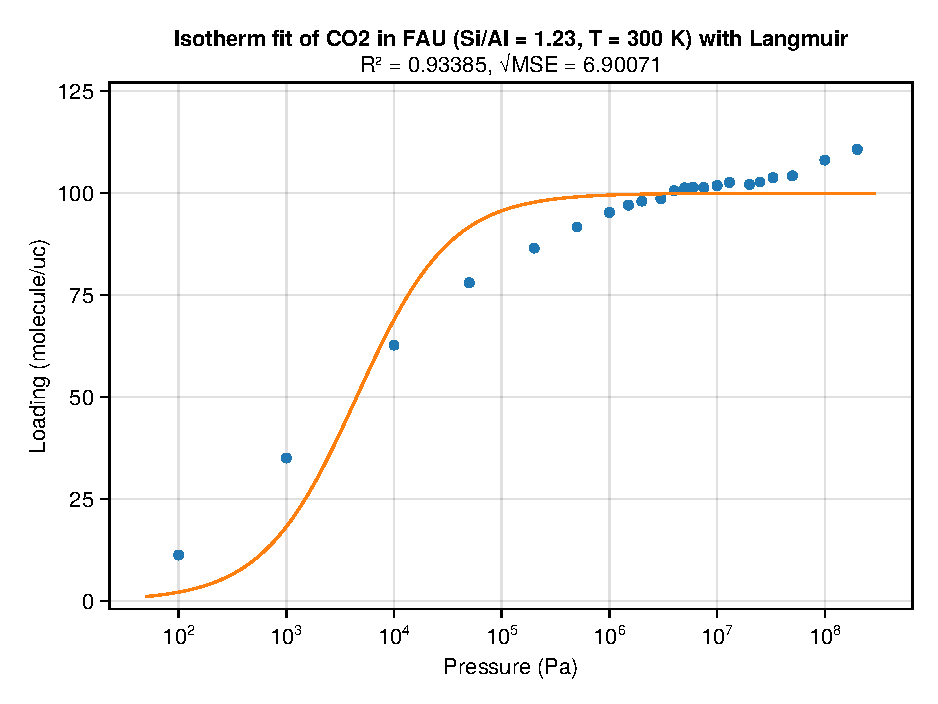
\includegraphics[width=\columnwidth]{figures/isotherms/Langmuir.pdf}
	\end{minipage}\hfill%
	\begin{minipage}{0.49\columnwidth}
		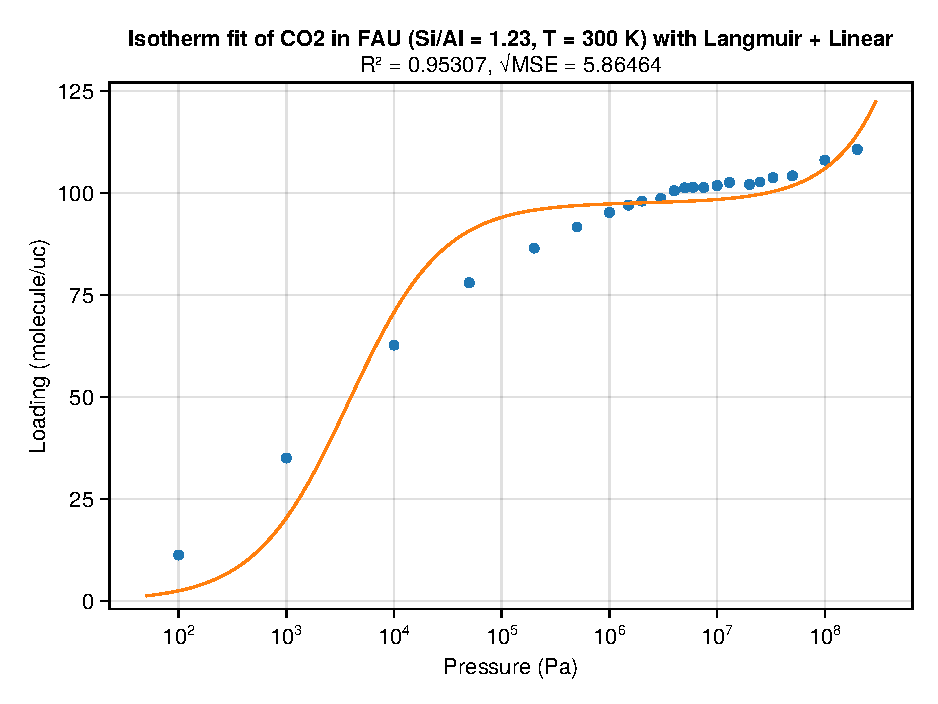
\includegraphics[width=\columnwidth]{figures/isotherms/Langmuir + Linear.pdf}
	\end{minipage}
	
	\begin{minipage}{0.49\columnwidth}
		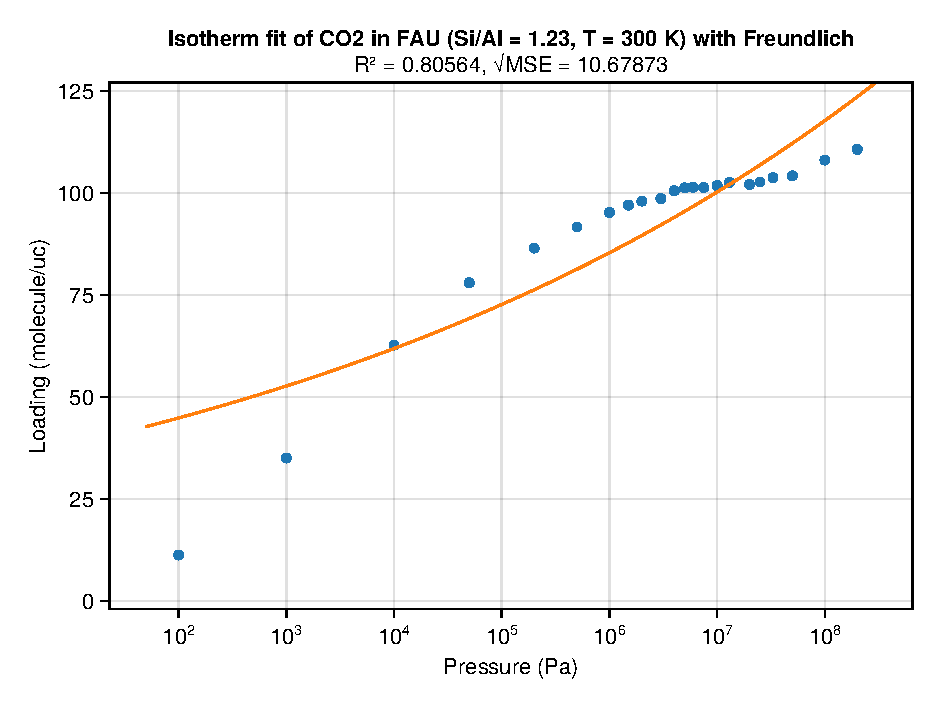
\includegraphics[width=\columnwidth]{figures/isotherms/Freundlich.pdf}
	\end{minipage}\hfill%
	\begin{minipage}{0.49\columnwidth}
		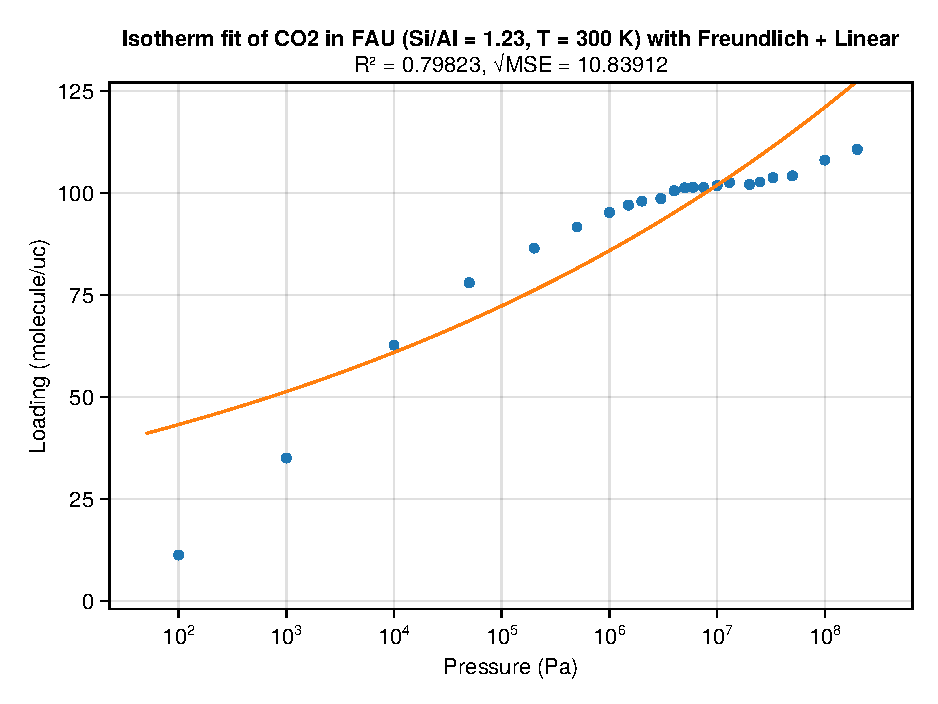
\includegraphics[width=\columnwidth]{figures/isotherms/Freundlich + Linear.pdf}
	\end{minipage}
	
	\begin{minipage}{0.49\columnwidth}
		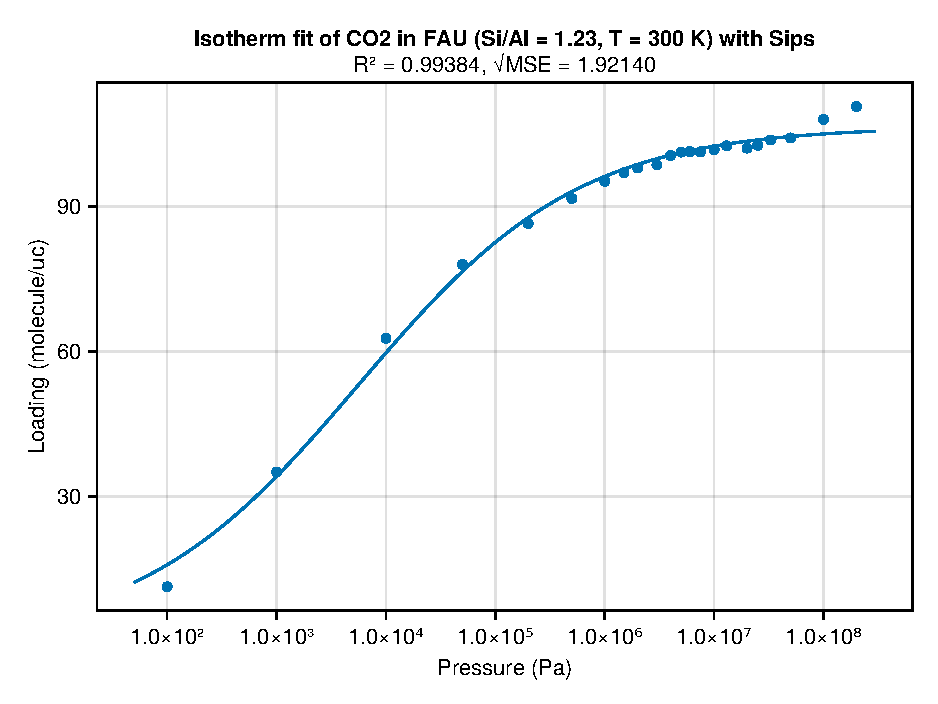
\includegraphics[width=\columnwidth]{figures/isotherms/Sips.pdf}
	\end{minipage}\hfill%
	\begin{minipage}{0.49\columnwidth}
		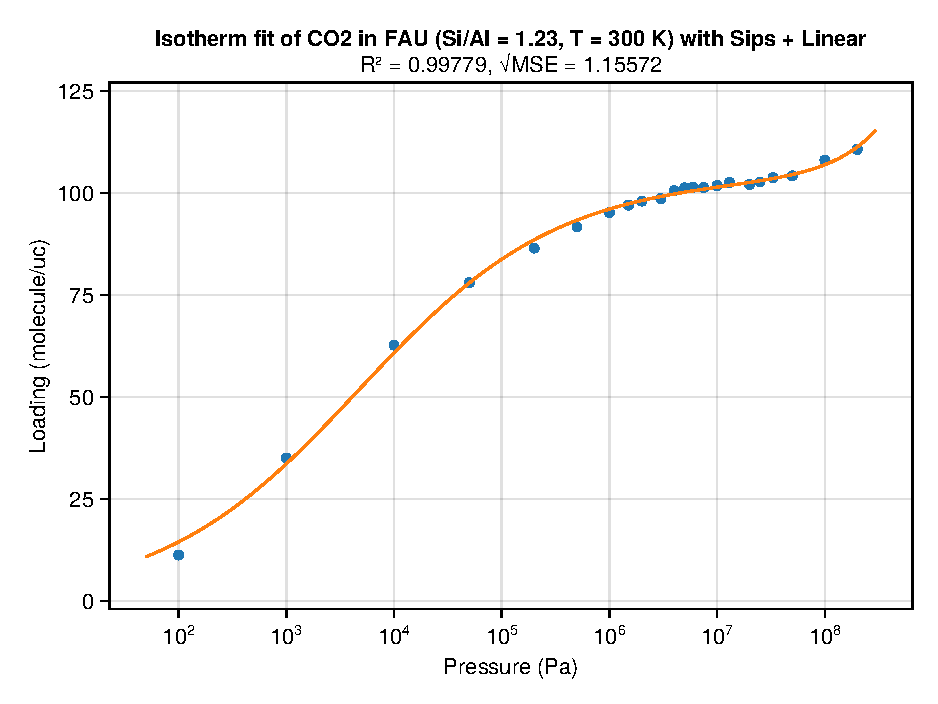
\includegraphics[width=\columnwidth]{figures/isotherms/Sips + Linear.pdf}
	\end{minipage}
	
	\begin{minipage}{0.49\columnwidth}
		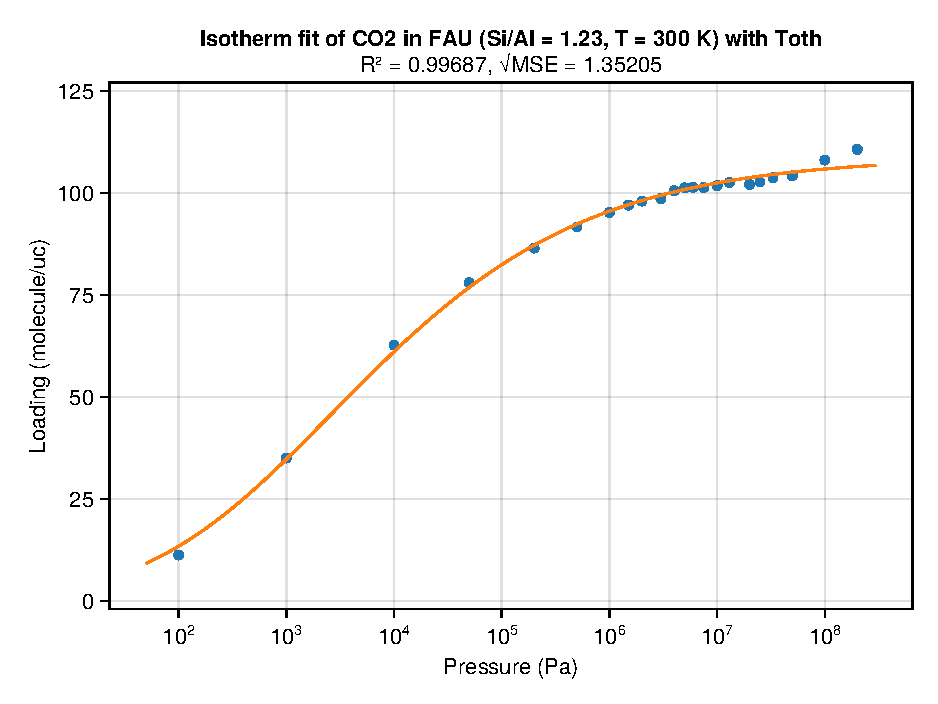
\includegraphics[width=\columnwidth]{figures/isotherms/Toth.pdf}
	\end{minipage}\hfill%
	\begin{minipage}{0.49\columnwidth}
		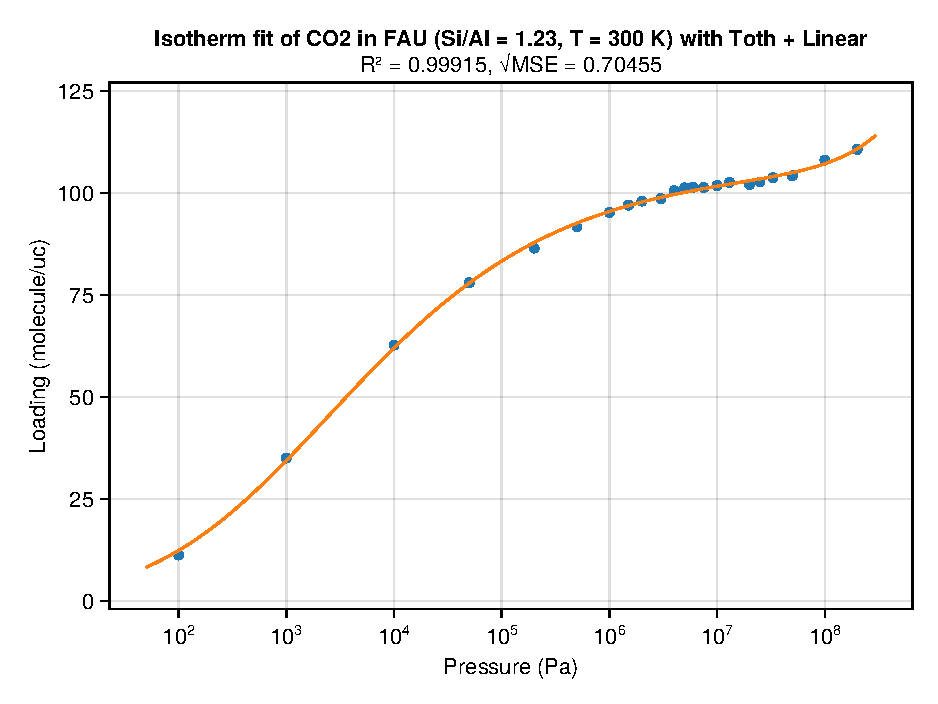
\includegraphics[width=\columnwidth]{figures/isotherms/Toth + Linear.pdf}
	\end{minipage}
	\caption{Simulated adsorption isotherm fitted with different models}\label{isothermfit}
\end{figure}

\begin{figure}\ContinuedFloat
	\begin{minipage}{0.49\columnwidth}
		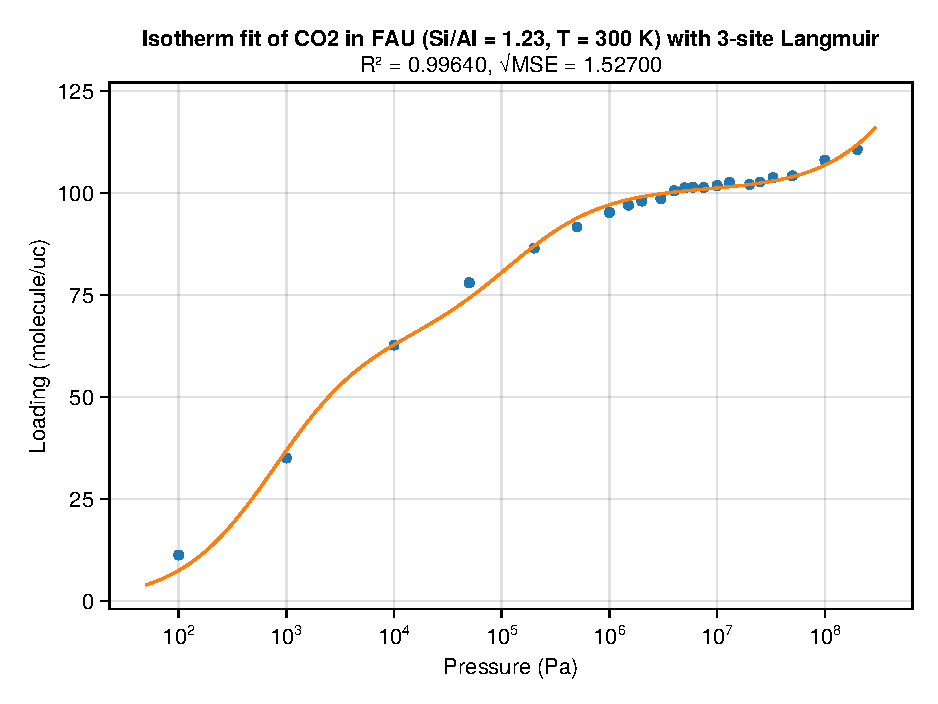
\includegraphics[width=\columnwidth]{figures/isotherms/3-site Langmuir.pdf}
	\end{minipage}\hfill%
	\begin{minipage}{0.49\columnwidth}
		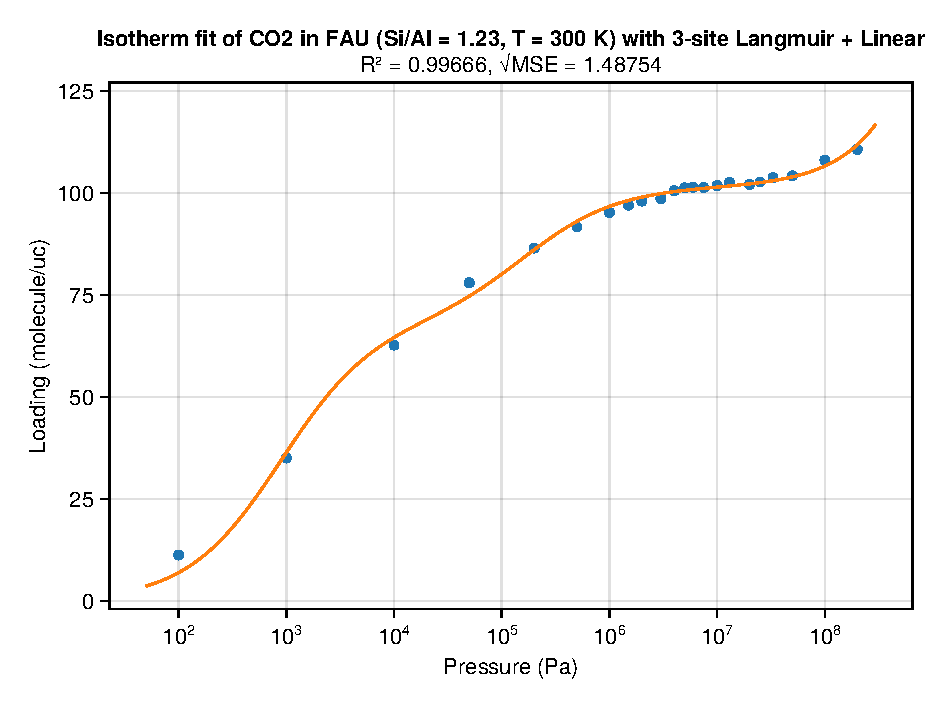
\includegraphics[width=\columnwidth]{figures/isotherms/3-site Langmuir + Linear.pdf}
	\end{minipage}
	
	\begin{minipage}{0.49\columnwidth}
		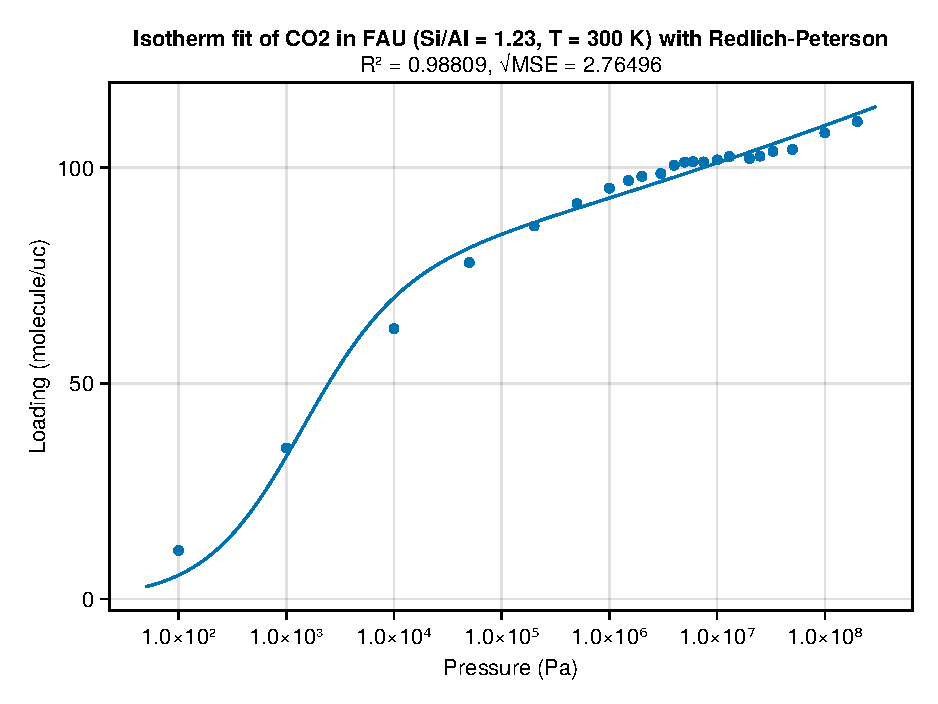
\includegraphics[width=\columnwidth]{figures/isotherms/Redlich-Peterson.pdf}
	\end{minipage}\hfill%
	\begin{minipage}{0.49\columnwidth}
		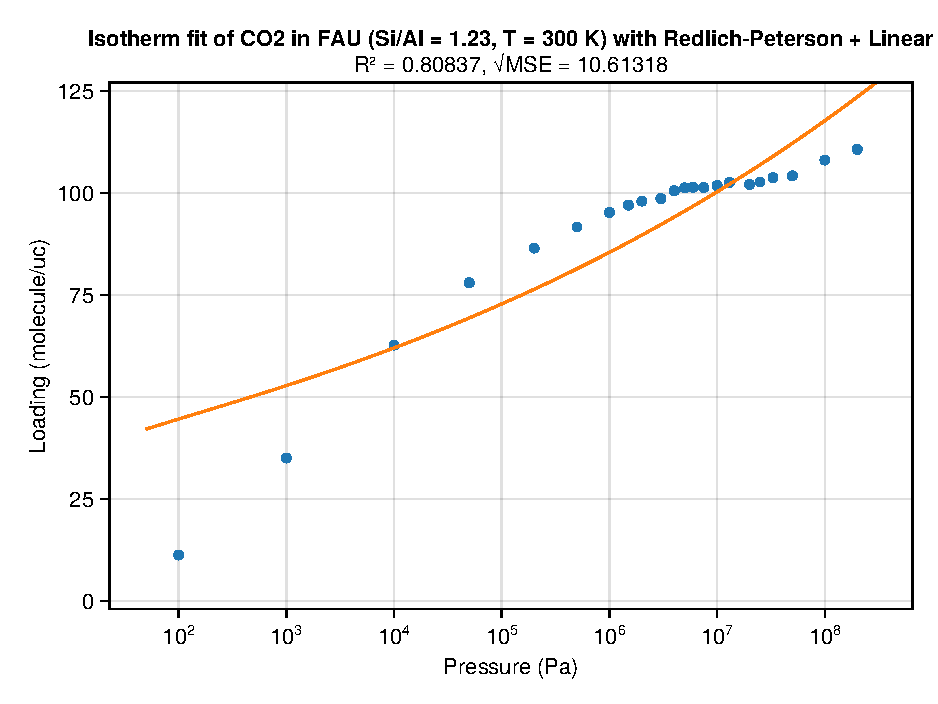
\includegraphics[width=\columnwidth]{figures/isotherms/Redlich-Peterson + Linear.pdf}
	\end{minipage}
	
	\begin{minipage}{0.49\columnwidth}
		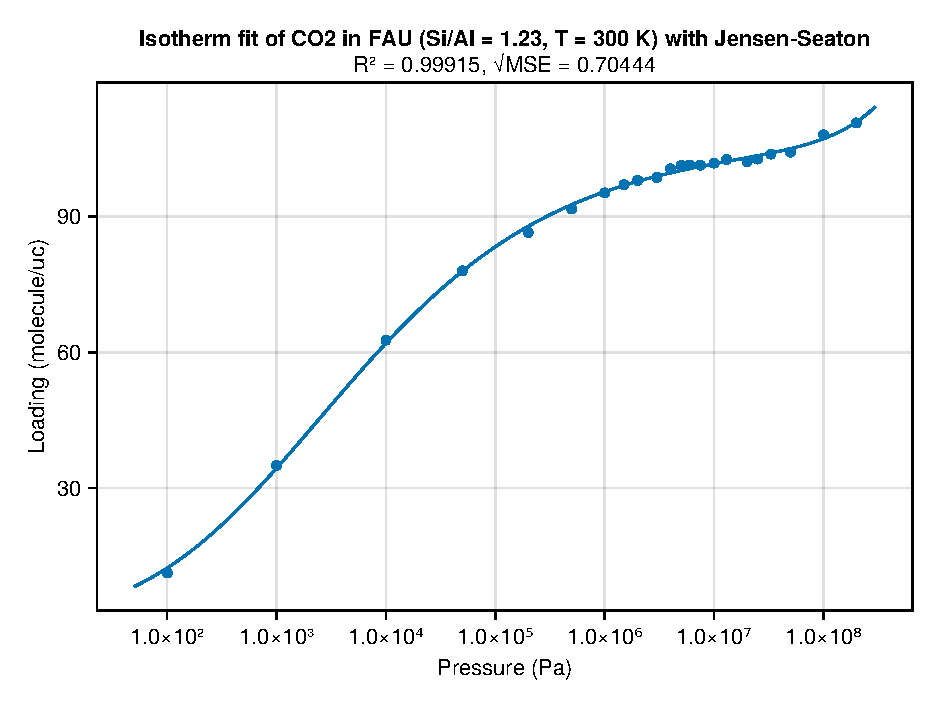
\includegraphics[width=\columnwidth]{figures/isotherms/Jensen-Seaton.pdf}
	\end{minipage}\hfill%
	\begin{minipage}{0.49\columnwidth}
		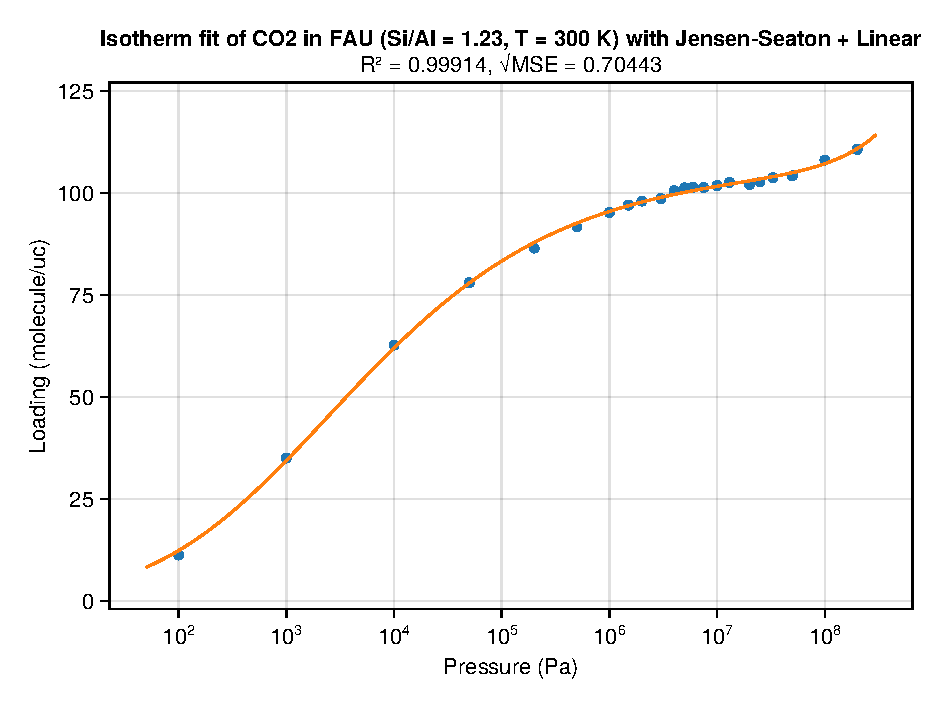
\includegraphics[width=\columnwidth]{figures/isotherms/Jensen-Seaton + Linear.pdf}
	\end{minipage}
	
	\begin{minipage}{0.49\columnwidth}
		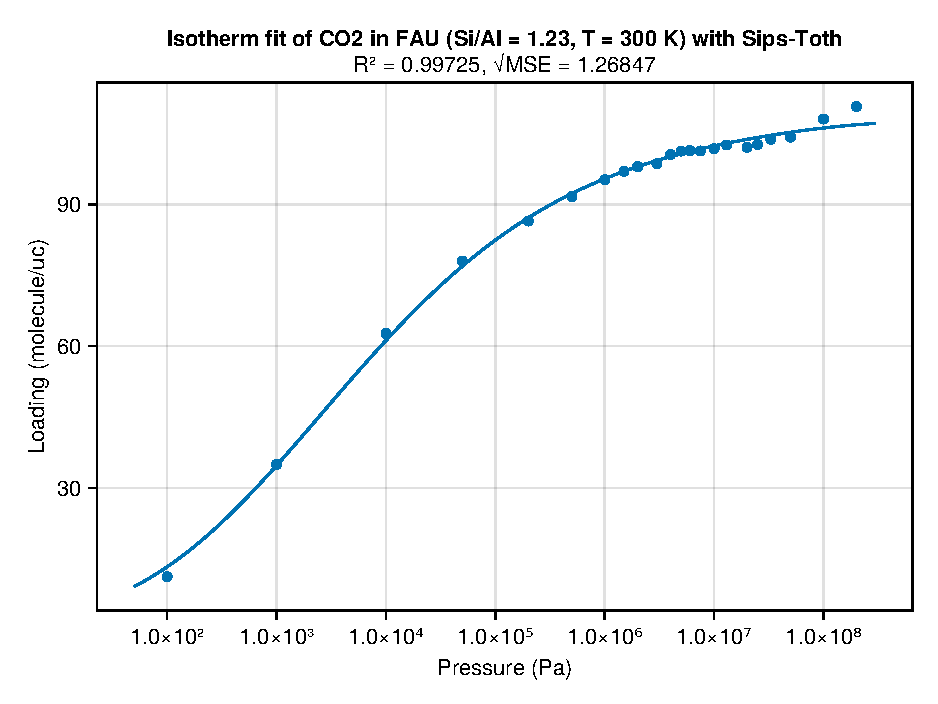
\includegraphics[width=\columnwidth]{figures/isotherms/Sips-Toth.pdf}
	\end{minipage}\hfill%
	\begin{minipage}{0.49\columnwidth}
		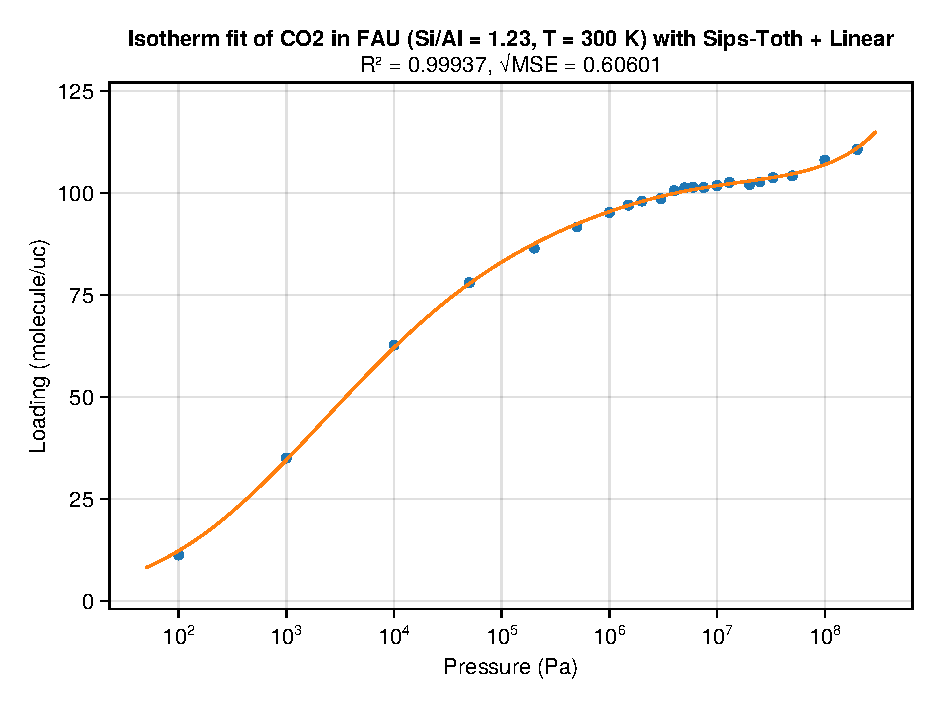
\includegraphics[width=\columnwidth]{figures/isotherms/Sips-Toth + Linear.pdf}
	\end{minipage}
	\caption{Simulated adsorption isotherm fitted with different models (continued)}
\end{figure}

The quality of the fit generally increases with the number of parameters, simply because of the increased flexibility of the model. Similarly, adding one extra linear parameter improves the quality of the overall fit, in particular at high pressure, since it corresponds to the linear compressibility regime. The case of the Jensen-Seaton adsorption model complements this point: there is no improvement in the fit due to the linear parameter in that case, because Jensen-Seaton isotherms already behave linearly at high pressure.

However, not all models perform equivalently. For example, even with 3 sites and thus 6 parameters, Langmuir fits very poorly compared to the Sips-Toth model plus linear term, which is the overall best and require one less parameter. With only 4 parameters, Toth plus linear is equivalent to Jensen-Seaton. Both Freundlich and Redlich-Peterson fail to fit because of the polynomial behaviour at high pressure. 

Other isotherms of the database generally leads to the same ordering of fit quality, so the most appropriate adsorption models to use for the current purpose seem to be either Jensen-Seaton (4 parameters) or Sips-Toth plus linear (5 parameters). The next subsection presents a simple statistical methodology to predict the values of the parameters of a model, whichever it may be, hence it is assumed that one adsorption model has been chosen and fixed.

\subsection{Simple meta-models}

Once a sufficient number of fitted isotherms are available, the next goal is to somehow interpolate across them across \SiAl ratio and temperatures for a given topology. Through fitting, this problem is reduced to finding function $\alpha(r, T)$, $\beta(r, T)$, $\gamma(r, T)$, \ldots \textit{i.e.} to expressing each parameter of the adsorption model as a function of the \SiAl ratio $r$ and the temperature $T$.

For each parameter $p$, I tried to express $p(r, T)$ through a simple meta-model -- \textit{i.e.} a model of the evolution of a (sub-)model parameter --, using \texttt{GLM.jl}, a Julia package for fitting linear models. In detail, I tried to fit expressions of the form
\[\der fp_p(p) = \der Ap\times \der fp_r(r) + \der Bp\times \der fp_T(T) + \der Cp\]
where each function $\der fp$ was either the identity, the inverse, or the log. Such a fit consists in finding the optimal parameters $\der Ap$, $\der Bp$ and $\der Cp$ to minimize the RMSD between both sides of the expected equality. There are 27 such expressions to test for each parameter $p$ since each of the three function $\der fp$ has three choices (identity, inverse, log), and the expression which yields the lowest RMSD is kept as the meta-model, along with the corresponding parameters.

For example, using the Jensen-Seaton adsorption model for \ce{CO_2} adsorption in FAU zeolites, the following expression is found for the $\beta$ parameter:
\[\log \beta(r, T) = - 1.8489\times\log r + 5170.7\times\frac1T -22.928 \label{eq:beta_fit_JS}\]

\begin{figure}
	\begin{subfigure}{0.49\columnwidth}
		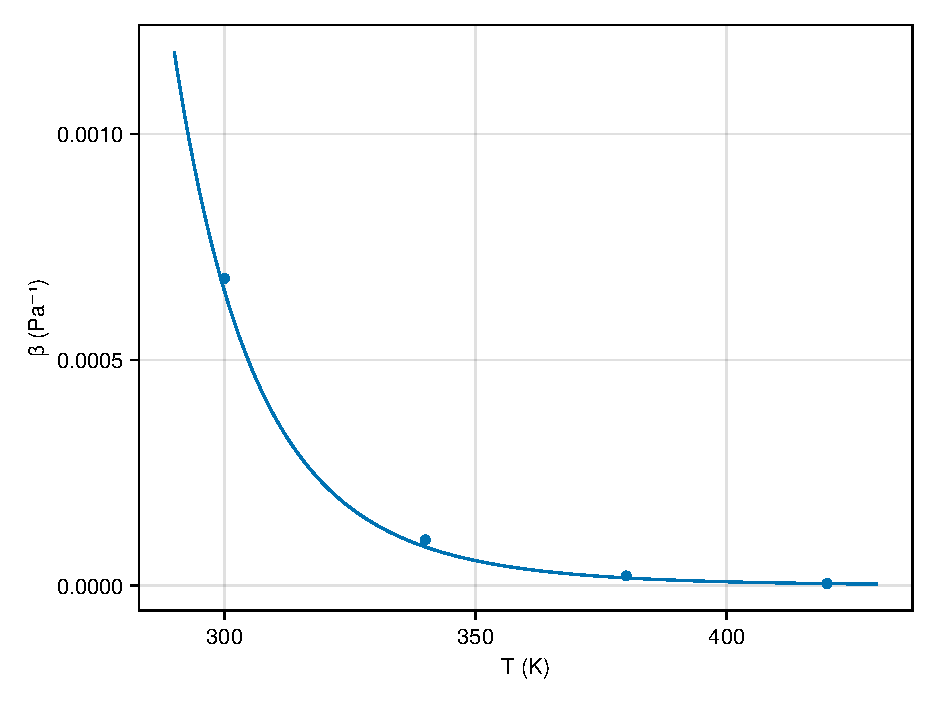
\includegraphics[width=\columnwidth]{figures/isotherms/evolution_beta_temperature.pdf}
		\subcaption{Evolution with temperature for Si/Al $= 2.43$}\label{subfig:beta_temperature}
	\end{subfigure}\hfill%
	\begin{subfigure}{0.49\columnwidth}
		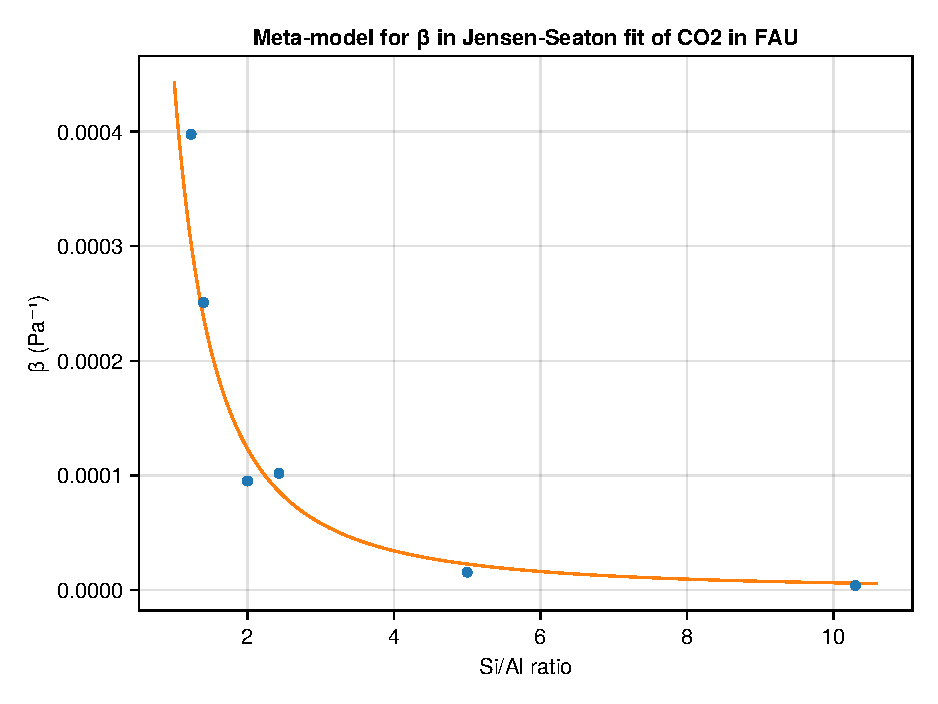
\includegraphics[width=\columnwidth]{figures/isotherms/evolution_beta_ratio.pdf}
		\subcaption{Evolution with Si/Al ratio for $T = \qty{340}K$}\label{subfig:beta_ratio}
	\end{subfigure}
	\caption{Evolution of the $\beta$ parameter in the Jensen-Seaton fit of \ce{CO_2} adsorption isotherms on FAU. The full line is the simple meta-model obtained in \cref{eq:beta_fit_JS}.}\label{fig:beta_evolution}
\end{figure}

\Cref{fig:beta_evolution} represents the comparison between the interpolated value of $\beta(r, T)$ and the values collected from the isotherms fitting in the previous setting. In this case, the fit works well, but the simple meta-model above does not always provide such a good level of agreement.

Overall, this approach provides a simple meta-model which works reasonably well to interpolate isotherms. For example, \cref{fig:simplemodelfit} shows the difference in quality between the direct Jensen-Seaton fit of an isotherm, and the one obtained from the simple meta-model. In this example, the simple meta-model was built using \SiAl ratios of 1, 1.23, 1.4, 2, 5 and 10 and temperatures of \qty{300}K, \qty{340}K and \qty{420}K, thus excluding the investigated point with \SiAl ratio of 2.4 at $T = \qty{380}K$. While not as quantitative as the actual fit, the simple meta-model allows retrieving an isotherm which is close to the reference without needing any additional computation.

\begin{figure}
	\begin{subfigure}{0.49\columnwidth}
		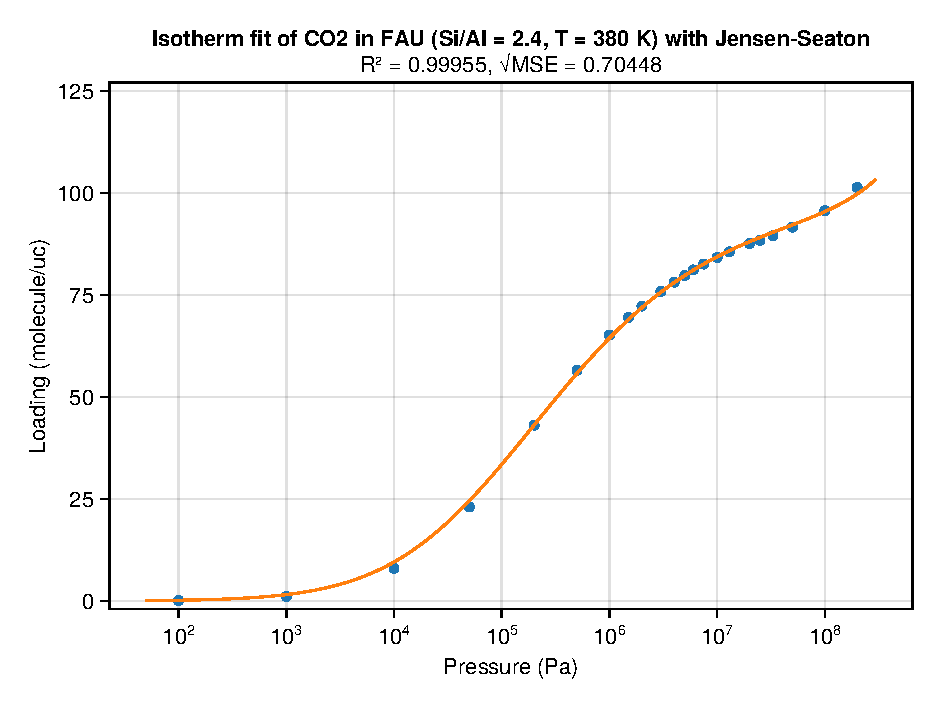
\includegraphics[width=\columnwidth]{figures/isotherms/referencefit_jsfit.pdf}
		\subcaption{Direct Jensen-Seaton fit}
	\end{subfigure}\hfill%
	\begin{subfigure}{0.49\columnwidth}
		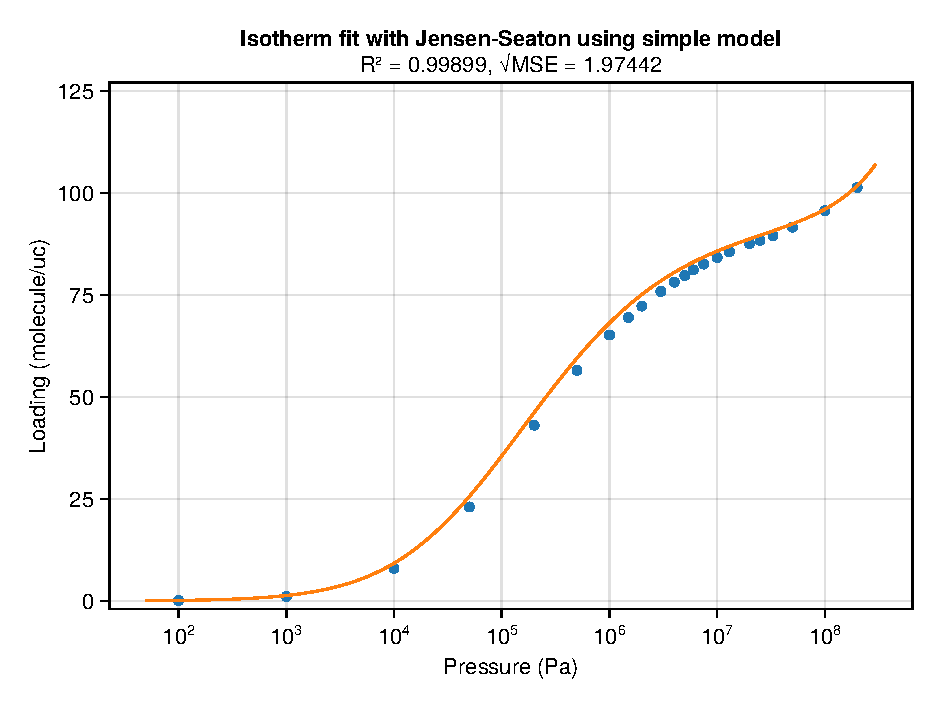
\includegraphics[width=\columnwidth]{figures/isotherms/referencefit_simplemodel.pdf}
		\subcaption{Interpolated fit using simple meta-model}
	\end{subfigure}
	\caption{Fitted adsorption isotherms of \ce{CO_2} in FAU with \SiAl = 2.4 at $T = \qty{380}K$}\label{fig:simplemodelfit}
\end{figure}

\section{Perspectives}

At the time of writing, I have only computed gas adsorption isotherms on three topologies: CHA, LTA and FAU. The previous methodology using simple meta-models to interpolate isotherms constitute a convenient method to obtain adsorption capacities given enough data for the target topology, but does not allow generalizing to other topologies. To reach this target, more isotherm data is required on various topologies, from which point it would become possible to create yet another simple meta-meta-model whose target are the coefficients $A$, $B$ and $C$ of the previous simple meta-model, depending only on the topology.

Another approach consists in relying on the more general tools of machine learning, instead of the custom approach detailed before. Deep learning could be used as a black-box method to directly learn the $p(r, T, \tau)$ functions, where $\tau$ designates the framework topology, numerically represented using ring statistics or coordination sequences for instance. Yet, once again, this requires much more isotherm data than what is currently available.

Fortunately, my cationic zeolite structure database now contains 64 topologies with representative structures across \SiAl ratios. Once the adsorption isotherms are computed on all of these structures, it should provide enough data to start creating a more robust predictive model.


\end{document}
